% Created 2019-01-13 Sun 12:50
% Intended LaTeX compiler: pdflatex
\documentclass[xcolor=table,10pt,aspectratio=169]{beamer}
\usepackage{graphicx}
\usepackage{grffile}
\usepackage{longtable}
\usepackage{wrapfig}
\usepackage{rotating}
\usepackage[normalem]{ulem}
\usepackage{amsmath}
\usepackage{textcomp}
\usepackage{amssymb}
\usepackage{capt-of}
\usepackage{hyperref}
\usepackage{microtype}
\usepackage{newunicodechar}
\usepackage[notions,operators,sets,keys,ff,adversary,primitives,complexity,asymptotics,lambda,landau,advantage]{cryptocode}
\usepackage{xspace}
\usepackage{units}
\usepackage{nicefrac}
\usepackage{gensymb}
\usepackage{amsthm}
\usepackage{amsmath}
\usepackage{amssymb}
\usepackage{xcolor}
\usepackage{listings}
\usepackage[color=yellow!40]{todonotes}
\RequirePackage{etex}
\RequirePackage[l2tabu,orthodox]{nag}            %% Warn about obsolete commands and packages
\RequirePackage{amsmath,amsfonts,amssymb,amsthm} %% Math
\RequirePackage{ifxetex,ifluatex}                %% Detect XeTeX and LuaTeX
\RequirePackage{fixltx2e}                        %% provides \textsubscript
\RequirePackage{xspace}
\RequirePackage{graphicx}
\RequirePackage{comment}
\RequirePackage{url}
\RequirePackage{relsize}
\RequirePackage{booktabs}
\RequirePackage{tabularx}
\RequirePackage[normalem]{ulem}
\RequirePackage[all]{xy}
\RequirePackage{etoolbox}

%%%
%%% Code Listings
%%%

\RequirePackage{listings}
\lstdefinelanguage{Sage}[]{Python}{morekeywords={True,False,sage,cdef,cpdef,ctypedef,self},sensitive=true}

\lstset{frame=none,
  showtabs=False,
  showspaces=False,
  showstringspaces=False,
  commentstyle={\color{gray}},
  keywordstyle={\color{mLightBrown}\textbf},
  stringstyle ={\color{mDarkBrown}},
  frame=single,
  basicstyle=\tt\scriptsize\relax,
  backgroundcolor=\color{gray!190!black},
  inputencoding=utf8,
  literate={…}{{\ldots}}1,
  belowskip=0.0em,
}

\makeatletter
\patchcmd{\@verbatim}
  {\verbatim@font}
  {\verbatim@font\scriptsize}
  {}{}
\makeatother

%%%
%%% Tikz
%%%

\RequirePackage{tikz,pgfplots}

\usetikzlibrary{calc}
\usetikzlibrary{arrows}
\usetikzlibrary{automata}
\usetikzlibrary{positioning}
\usetikzlibrary{decorations.pathmorphing}
\usetikzlibrary{backgrounds}
\usetikzlibrary{fit,}
\usetikzlibrary{shapes.symbols}
\usetikzlibrary{chains}
\usetikzlibrary{shapes.geometric}
\usetikzlibrary{shapes.arrows}
\usetikzlibrary{graphs}

%%%
%%% SVG (Inkscape)
%%%

\ifxetex % chktex 1
\newcommand{\executeiffilenewer}[3]{%
  {\immediate\write18{#3}} % hack
}
\else
\newcommand{\executeiffilenewer}[3]{%
  \ifnum\pdfstrcmp{\pdffilemoddate{#1}}%
    {\pdffilemoddate{#2}}>0%
    {\immediate\write18{#3}}
  \fi%
}
\fi

\newcommand{\includesvg}[2][1.0\textwidth]{%
 \executeiffilenewer{#1.svg}{#1.pdf}%
 {inkscape -z -D --file=#2.svg --export-pdf=#2.pdf --export-latex --export-area-page}%
 \def\svgwidth{#1} 
 \input{#2.pdf_tex}%
} 

%%%
%%% Metropolis Theme
%%%

\usetheme{metropolis}
\metroset{color/block=fill}
\metroset{numbering=none}
\metroset{outer/progressbar=foot}
\metroset{titleformat=smallcaps}

\setbeamercolor{description item}{fg=mLightBrown}
% \setbeamerfont{alerted text}{series=\bfseries}
\setbeamerfont{footnote}{size=\scriptsize}
\setbeamercolor{example text}{fg=mDarkBrown}
\setbeamercolor{block title alerted}{fg=white, bg=mDarkBrown}
\setbeamertemplate{bibliography item}[text]

\renewcommand*{\UrlFont}{\ttfamily\relax}

%%%
%%% UTF-8 & Fonts
%%% 

\RequirePackage{unicodesymbols} % after metropolis which loads fontspec

\setmonofont[BoldFont={Cousine Bold},
             ItalicFont={Cousine Italic},
             BoldItalicFont={Cousine Bold Italic},
             Scale=0.9]{Cousine}             
%%%
%%% BibLaTeX
%%%

\RequirePackage[backend=bibtex,
            style=alphabetic,
            maxnames=10,
            citestyle=alphabetic]{biblatex}

\bibliography{local.bib,abbrev3.bib,crypto_crossref.bib,rfc.bib,jacm.bib}

\DeclareFieldFormat{title}{\alert{#1}}
\DeclareFieldFormat[book]{title}{\alert{#1}}
\DeclareFieldFormat[thesis]{title}{\alert{#1}}
\DeclareFieldFormat[inproceedings]{title}{\alert{#1}}
\DeclareFieldFormat[incollection]{title}{\alert{#1}}
\DeclareFieldFormat[article]{title}{\alert{#1}}
\DeclareFieldFormat[misc]{title}{\alert{#1}}

%%% 
%%% Microtype
%%%

\IfFileExists{upquote.sty}{\RequirePackage{upquote}}{}
\IfFileExists{microtype.sty}{\RequirePackage{microtype}}{}

\setlength{\parindent}{0pt}                   %%
\setlength{\parskip}{6pt plus 2pt minus 1pt}  %%
\setlength{\emergencystretch}{3em}            %% prevent overfull lines
\setcounter{secnumdepth}{0}                   %%

\let\nl\undefine
\let\procedure\relax
\let\endprocedure\relax

\usepackage{algorithm2e}
\renewcommand{\vec}[1]{\mathbf{#1}\xspace}
\newcommand{\mat}[1]{\mathbf{#1}\xspace}

\definecolor{DarkPurple}{HTML}{332288}
\definecolor{DarkBlue}{HTML}{6699CC}
\definecolor{LightBlue}{HTML}{88CCEE}
\definecolor{DarkGreen}{HTML}{117733}
\definecolor{DarkRed}{HTML}{661100}
\definecolor{LightRed}{HTML}{CC6677}
\definecolor{LightPink}{HTML}{AA4466}
\definecolor{DarkPink}{HTML}{882255}
\definecolor{LightPurple}{HTML}{AA4499}
\definecolor{DarkBrown}{HTML}{604c38}
\definecolor{DarkTeal}{HTML}{23373b}
\definecolor{LightBrown}{HTML}{EB811B}
\definecolor{LightGreen}{HTML}{14B03D}
\definecolor{DarkOrange}{HTML}{FFDD00}

\pgfplotsset{width=1.0\textwidth,
  height=0.6\textwidth,
  xlabel={$\beta$},
  ylabel={$\log_{2}(\#\textnormal{nodes})$},
  cycle list={%
    solid,LightGreen,thick\\%
    dotted,LightRed,very thick\\%
    dashed,DarkBlue,thick\\%
    dashdotted,DarkPink,thick\\%
    dashdotdotted,LightGreen,thick\\%
    loosely dotted,very thick\\%
    loosely dashed,DarkBlue,very thick\\%
    loosely dashdotted,DarkPink,very thick\\%
    \\%
    DarkBrown,thick\\%
  },
  legend pos=north west,
  legend cell align={left}}

\pgfplotsset{select coords between index/.style 2 args={
    x filter/.code={
        \ifnum\coordindex<#1\def\pgfmathresult{}\fi
        \ifnum\coordindex>#2\def\pgfmathresult{}\fi
    }
}}


%%% Local Variables:
%%% mode: latex
%%% End:
\def\enumquadfit{\(0.000784314\, \beta^2 + 0.366078\,\beta - 6.125\)}
\def\enumlinfit{\(0.18728\, \beta \log(\beta) - 1.0192\,\beta + 16.10\)}
\def\robl{\rowcolor{DarkBlue!20}}
\def\rore{\rowcolor{DarkRed!20}}
\def\rogr{\rowcolor{gray!20}}
\usetheme{default}
\author{Martin R. Albrecht \alert{@martinralbrecht}}
\date{10 January 2019, RWC\vfill \begin{scriptsize}Based on joint work with Alex Davidson, Amit Deo, Benjamin R. Curtis, Eamonn W. Postlethwaite, Elena Kirshanova, Fernando Virdia, Florian Göpfert, Gottfried Herold, Léo Ducas, Marc Stevens, Rachel Player, Sam Scott and Thomas Wunderer as well as the work of many other authors.\end{scriptsize}}
\title{So how hard is solving LWE/NTRU anyway?}
\hypersetup{
pdfauthor={Martin R. Albrecht \alert{@martinralbrecht}},
pdftitle={So how hard is solving LWE/NTRU anyway?},
pdfkeywords={},
pdfsubject={},
pdfcreator={Emacs 26.1 (Org mode 9.2)},
pdflang={English},
colorlinks,
citecolor=gray,
filecolor=gray,
linkcolor=gray,
urlcolor=gray
}
\begin{document}

\maketitle

\section{Introduction}
\label{sec:org2eea74b}
\begin{frame}[label={sec:org21eba80}]{NIST Process: Selected Non-Quantum Security Estimates}
\rowcolors[]{3}{gray!20}{gray!10}

\begin{center}
\small{
\begin{tabular}{rrrrrr}
\textbf{Scheme}      / & \textbf{Kyber} & \textbf{Lima} & \textbf{R EMBLEM} & \textbf{NTRU HRSS} & \textbf{SNTRU'}\\
\textbf{Cost Model} &  &  &  &  & \\
\hline
\textbf{Kyber}\footnotemark & 180 & 218 & 112 & 136 & 155\\
\textbf{Lima}\footnotemark & 196 & 234 & 129 & 152 & 171\\
\textbf{R EMBLEM}\footnotemark & 210 & 248 & 142 & 165 & 184\\
\textbf{NTRU HRSS}\footnotemark & 456 & 587 & 242 & 313 & 370\\
\textbf{SNTRU’}\footnotemark & 535 & 722 & 270 & 350 & 410\\
\end{tabular}
\footnotetext[1]{\label{orga96acda}\(0.292\beta\) \cite{USENIX:ADPS16}, \alert{this is an explicit underestimate}}\footnotetext[2]{\label{orgea1fe74}\(0.292\beta + 16.4\) \cite{NISTPQC-R1:LIMA17}, \alert{this is a somewhat explicit underestimate}}\footnotetext[3]{\label{org2bb654d}\(0.292\beta + \log(8d) + 16.4\) \cite{JMC:AlbPlaSco15}}\footnotetext[4]{\label{org05d0355}\enumlinfit{} \(+ 7\) \cite{JMC:AlbPlaSco15}}\footnotetext[5]{\label{org30742d0}\enumquadfit{} \(\log(8d) + 7\) \cite{EPRINT:HPSSWZ15a}}
}
\end{center}

\scriptsize{
Source: \fullcite{SCN:ACDDPP18}, \url{https://estimate-all-the-lwe-ntru-schemes.github.io/docs/}
}

\vspace{1em}
\end{frame}

\begin{frame}[label={sec:orgb43d3e5}]{Learning with Errors}
Given \((\mathbf{A},\vec{c})\), find \(\vec{s}\) when

\[
\left(\begin{array}{c}
\\
\\
\\ 
\vec{c} \\
\\
\\
\\
\end{array} \right) \equiv \left(
\begin{array}{ccc}
\leftarrow & n & \rightarrow \\
\\
\\ 
& \mathbf{A} & \\
\\
\\
\\
\end{array} \right) \cdot \left( \begin{array}{c}
\\\
\\
\vec{s} \\
\\
\\
\end{array} \right) + \left(
\begin{array}{c}
\\
\\
\\ 
\vec{e} \\
\\
\\
\\
\end{array} 
\right)
\]

for \(\vec{c} \in \ZZ_q^{m}\), \(\mathbf{A} \in \ZZ_q^{m \times n}\), and \(\vec{s} \in \ZZ^{n}\) and \(\vec{e} \in \ZZ^{m}\) having small coefficients.
\end{frame}

\section{Primal Attack}
\label{sec:orge3deaa9}
\begin{frame}[label={sec:org1ff70a7}]{Unique SVP Approach}
We can reformulate \(\vec{c} - \mathbf{A} \cdot \vec{s} \equiv \vec{e} \bmod q\)  over the Integers as:
\[
  \begin{pmatrix}
    q\mathbf{I} & -\mathbf{A}\\
    0 & \mathbf{I}\\
  \end{pmatrix} \cdot
  \begin{pmatrix}
    \mathbf{*}\\
    \mathbf{s}
  \end{pmatrix} +
  \begin{pmatrix}
    \vec{c}\\
    \vec{0}
  \end{pmatrix} = 
  \begin{pmatrix}
    \vec{e}\\
    \vec{s}
  \end{pmatrix}
\]
Alternatively:
\[
  \mathbf{B} = \begin{pmatrix}
    q\mathbf{I} & -\mathbf{A} & \vec{c}\\
    0 & \mathbf{I} & 0\\
    0 & 0 & 1\\
  \end{pmatrix}, \qquad
  \mathbf{B} \cdot
  \begin{pmatrix}
    \vec{*}\\
    \vec{s}\\
    1
  \end{pmatrix} = 
  \begin{pmatrix}
    \vec{e}\\
    \vec{s}\\
    1
  \end{pmatrix}
\]

In other words, there exists an integer-linear combination of the columns of \(\mathbf{B}\) that produces a vector with “unusually” small coefficients \(\rightarrow\) a unique shortest vector.
\end{frame}

\begin{frame}[label={sec:orga9725b3}]{Computational Problem}
\begin{block}{Unique Shortest Vector Problem}
Find a unique shortest vector amongst the integer combinations of the columns of:
\[
  \mathbf{B} = \begin{pmatrix}
    q\mathbf{I} & -\mathbf{A} & \vec{c}\\
    0 & \mathbf{I} & 0\\
    0 & 0 & 1\\
  \end{pmatrix}
\]
where \(\mat{B} \in \ZZ^{d \times d}\).
\end{block}
\end{frame}

\section{Lattice Reduction}
\label{sec:orgea2cb8b}
\begin{frame}[label={sec:orga96d8be}]{Length of Gram-Schmidt Vectors}
It will be useful to consider the lengths of the Gram-Schmidt vectors.

The vector \(\vec{b}^*_i\) is the orthogonal projection of \(\vec{b}_i\) to the space spanned by the vectors \(\vec{b}_0, \ldots, \vec{b}_{i-1}\).

\begin{columns}
\begin{column}{0.45\columnwidth}
Informally, this means taking out the contributions in the directions of previous vectors  \(\vec{b}_0, \ldots, \vec{b}_{i-1}\).
\end{column}

\begin{column}{0.45\columnwidth}
\begin{tikzpicture}
\pgfplotsset{width=\textwidth, height=0.6\textwidth}
\draw[->] (0,0) -- (3,1);
\node[] at (3.2,1.2) {$\vec{b}_0$};
\only<1>{\draw[->] (0,0) -- (1,2);}
\only<1>{\node[] at (1.2,2.2) {$\vec{b}_1$};}
\only<2>{\draw[->,color=lightgray] (0,0) -- (1,2);}
\only<2>{\node[color=lightgray] at (1.2,2.2) {$\vec{b}_1$};}
\only<2>{\draw[->,gray] (0,0) -- (-0.5,1.5);}
\only<2>{\node[] at (-0.3,1.7) {$\vec{b}^*_1$};}
\only<1>{\node[] at (-0.3,1.7) {\phantom{$\vec{b}^*_1$}};}
\end{tikzpicture}
\end{column}
\end{columns}
\end{frame}

\begin{frame}[label={sec:orgcfc4eb4},fragile]{Example}
 \lstset{language=sage,label= ,caption= ,captionpos=b,numbers=none}
\begin{lstlisting}
sage: A = IntegerMatrix.random(120, "qary", k=60, bits=20)[::-1]
sage: M = GSO.Mat(A); M.update_gso()
sage: lg = [(i,log(r_, 2)/2) for i, r_ in enumerate(M.r())]
sage: line(lg, **plot_kwds)
\end{lstlisting}

\begin{center}
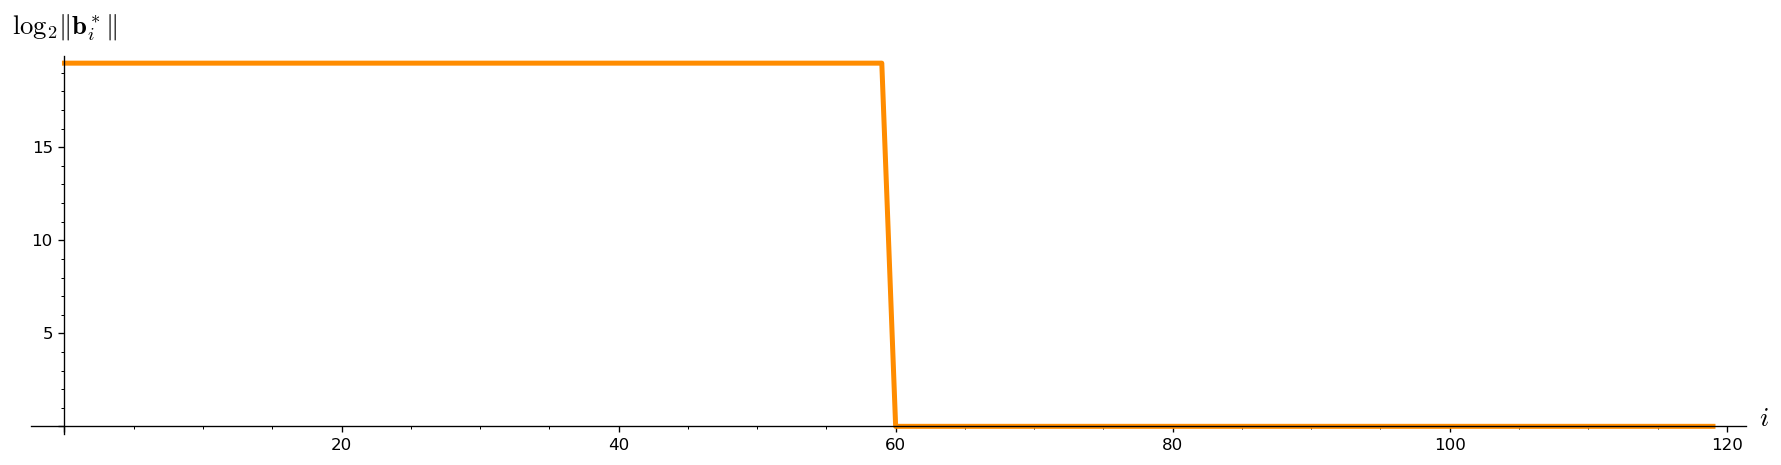
\includegraphics[width=.9\linewidth]{gram-schmidt-norms.png}
\end{center}
\end{frame}

\begin{frame}[label={sec:orge99c28a},fragile]{Example - LLL}
 \lstset{language=sage,label= ,caption= ,captionpos=b,numbers=none}
\begin{lstlisting}
sage: A = LLL.reduction(A)
sage: M = GSO.Mat(A); M.update_gso()
sage: lg = [(i,log(r_, 2)/2) for i, r_ in enumerate(M.r())]
sage: line(lg, **plot_kwds)
\end{lstlisting}

\begin{center}
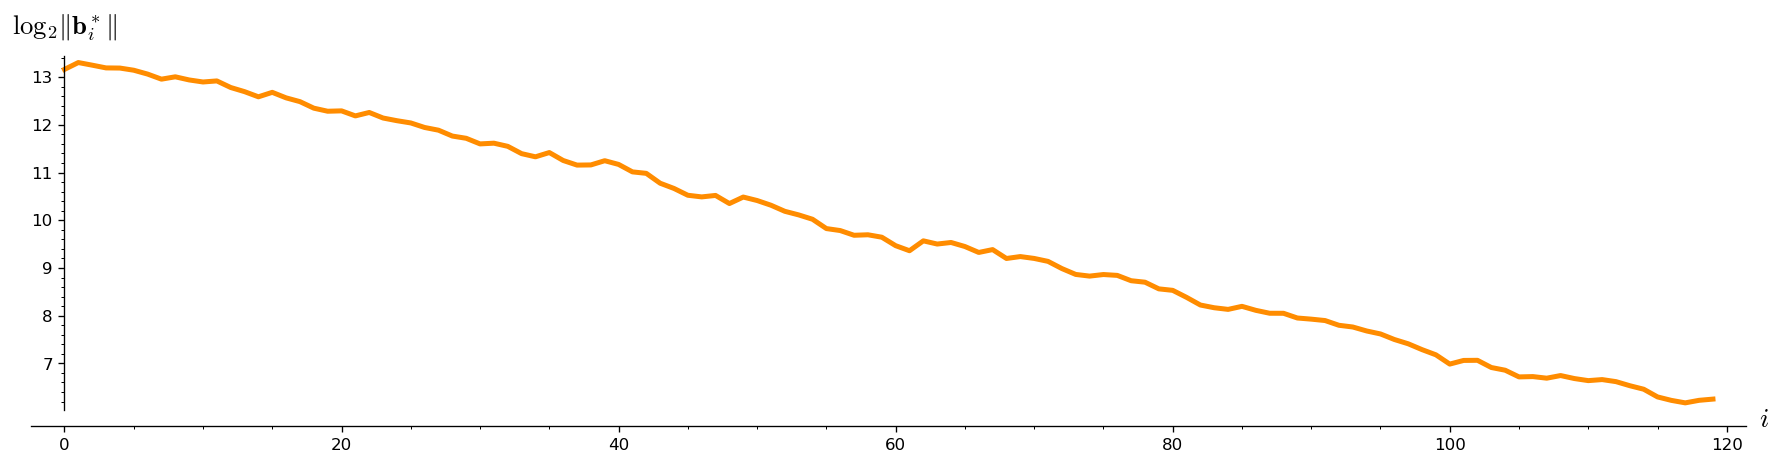
\includegraphics[width=.9\linewidth]{gram-schmidt-norms-lll.png}
\end{center}

\textbf{Geometric Series Assumption:} The shape after lattice reduction is a line with a flatter slope as lattice reduction gets stronger.
\end{frame}

\begin{frame}[label={sec:orgda3e633}]{Success Condition for uSVP}
\begin{tikzpicture}
\begin{axis}[/pgf/number format/.cd,fixed,ymin = 1,legend pos=north east,legend style={fill=white}, xlabel=,ylabel=$\log_2(\norm \cdot)$,width=\columnwidth, height=0.4\columnwidth, xmin = 1, xmax = 183,legend cell align=left,]
%      \draw[->] (-3,0) -- (4.2,0) node[right] {$x$};
%      \draw[->] (0,-3) -- (0,4.2) node[above] {$y$};
\addplot[domain=1:183,smooth,variable=\x,black] plot ({\x},{log2(1.01170246711949^(-2*(\x-1)+183)*54.5751087741536)});
\addlegendentry{GSA for $\norm{\vec b_i^*}$}

\addplot[domain=1:183,samples=1000, smooth,variable=\x,darkgray,dotted,thick] plot ({\x},{log2( 3.19153824321146 * sqrt(183 - \x + 1) )});

\addlegendentry{length of projection of $(\vec{e},\vec{s},1)$}

\draw[dashed] (127,1) -- (127,820) node[pos = 0.06, right] {$d-\beta+1$};
\end{axis}
\end{tikzpicture}

\scriptsize{

\fullcite{USENIX:ADPS16}

\fullcite{AC:AGVW17}

}
\end{frame}

\begin{frame}[label={sec:orgd70a89b}]{Slope}
The slope depends on the \textbf{root Hermite factor} \(\delta\) which depends on the “block size” \(\beta\).

\begin{tikzpicture}
\pgfplotsset{width=\textwidth, height=0.4\textwidth}

\begin{axis}[xlabel={$\beta$},ylabel={$\delta$},legend pos=north east, legend style={fill=none},  yticklabel style={/pgf/number format/fixed, /pgf/number format/precision=4}]
         	
\addplot[black, thick] coordinates {
(50, 1.01206486355485) (60, 1.01145310214785) (70, 1.01083849117278)
(80, 1.01026264533039) (90, 1.00973613406057) (100, 1.00925872103633)
(110, 1.00882653150498) (120, 1.00843474281592) (130, 1.00807860284815)
(140, 1.00775378902354) (150, 1.00745650119215) (160, 1.00718344897388)
(170, 1.00693180103572) (180, 1.00669912477197) (190, 1.00648332800111)
(200, 1.00628260691082) (210, 1.00609540127612) (220, 1.00592035664374)
(230, 1.00575629268952) (240, 1.00560217684407) (250, 1.00545710232739)
};
\addlegendentry{$(\frac{\beta}{2\pi e} \cdot (\pi\, \beta)^{1/\beta} )^{\frac{1}{2(\beta-1)}}$};

\end{axis}
\end{tikzpicture}

\small{

\fullcite{PhD:Chen13}

}
\end{frame}

\begin{frame}[label={sec:org58ffb3a}]{Strong Lattice Reduction: BKZ Algorithm}
\centering
\(
 \left(
     \begin{array}{ccccccccc}
                 &           &           &           &           &           &           &           &           \\
                 &           &           &           &           &           &           &           &           \\
                 &           &           &           &           &           &           &           &           \\
         \only<1-2>{\vec{b}_{0}}   \only<3->{{\color{LightRed} \vec{b}_{0}}}          &
         \only<1-5>{\vec{b}_{1}}   \only<6->{{\color{LightRed} \vec{b}_{1}}}          &
         \only<1-8>{\vec{b}_{2}}   \only<9->{{\color{LightRed} \vec{b}_{2}}}          &
         {\vec{b}_{3}}                                                             &
         {\vec{b}_{4}}                                                             &
         {\vec{b}_{5}}                                                             &
         {\vec{b}_{6}}                                                             &
         {\vec{b}_{7}}                                                             &
         \dots   \\
                 &           &           &           &           &           &           &           &           \\
                 &           &           &           &           &           &           &           &           \\
                 &           &           &           &           &           &           &           &
     \end{array}
        \right)
    \)
    \begin{tikzpicture}[remember picture, overlay]
      \tikzset{shift={(current page.center)},yshift=-1.5cm}
      \node[] at (0,0) (origin) {};
      {\color{DarkBlue} %
        \only<1-3>{%
          \draw (-.1,3) -- (-.1,2) {};
          \draw (-.1,1) -- (-.1,0) {};
          \draw (-3,3) -- (-3,2) {};
          \draw (-3,1) -- (-3,0) {};
          \draw[decorate,decoration={brace,amplitude=10pt}]
          (-3,3.2) -- (-.1,3.2) node [black,midway,yshift=.6cm]
          {$\beta = 5$};
          \only<2>{%
            \draw[decorate,decoration={brace,amplitude=10pt}]
            (-.1,-.2) -- (-3,-.2) {};
          }
        }
        \only<4-6>{%
          \draw (.6,3) -- (.6,2) {};
          \draw (.6,1) -- (.6,0) {};
          \draw (-2.3,3) -- (-2.3,2) {};
          \draw (-2.3,1) -- (-2.3,0) {};
          \draw[decorate,decoration={brace,amplitude=10pt}]
          (-2.3,3.2) -- (.6,3.2) node [black,midway,yshift=.6cm]
          {$\beta = 5$};
          \only<5>{%
            \draw[decorate,decoration={brace,amplitude=10pt}]
            (.6,-.2) -- (-2.3,-.2) {};
          }
        }
        \only<7-9>{%
          \draw (1.3,3) -- (1.3,2) {};
          \draw (1.3,1) -- (1.3,0) {};
          \draw (-1.6,3) -- (-1.6,2) {};
          \draw (-1.6,1) -- (-1.6,0) {};
          \draw[decorate,decoration={brace,amplitude=10pt}]
          (-1.6,3.2) -- (1.3,3.2) node [black,midway,yshift=.6cm]
          {$\beta = 5$};
          \only<8>{%
            \draw[decorate,decoration={brace,amplitude=10pt}]
            (1.3,-.2) -- (-1.6,-.2) {};
          }
        }
      }
      \node (oracle) at (-4,-1.8) {
\includegraphics[scale=0.9]{oracle.png}};
      \only<2>{%
        \draw[->] (-2.8,-.5) to[in=70,out=160] (-4,-.8);
        \draw[->] (-3,-2) to [in=270,out=20] (-0.5,-.5);
      }
      \only<5>{%
        \draw[->] (-2.1,-.5) to[in=70,out=160] (-4,-.8);
        \draw[->] (-3,-2) to [in=270,out=20] (.2,-.5);
      }
      \only<8>{%
        \draw[->] (-1.4,-.5) to[in=70,out=160] (-4,-.8);
        \draw[->] (-3,-2) to [in=270,out=20] (.2,-.5);      
      }
      \node at (5, -2.5) {\tiny{Picture credit: Eamonn Postlethwaite}};
\end{tikzpicture}
\end{frame}

\begin{frame}[label={sec:org3a6b1e6}]{BKZ Algorithm}
\begin{algorithm}[H]
  \KwData{LLL-reduced lattice basis \(\mat{B}\)}
  \KwData{block size \(\beta\)}
  \SetKwFor{MRepeat}{repeat}{}{}
  \MRepeat{until no more change}{
    \For{\(\kappa \gets 0\) \KwTo{} \(d-1\)}{
        LLL  on local projected block \([\kappa,\ldots,\kappa+\beta-1]\)\; 
        \(\vec{v} \gets \) find shortest vector in local projected block \([\kappa,\ldots,\kappa+\beta-1]\)\;
        insert $\vec{v}$ into $\vec{B}$\;
    }
  }
\end{algorithm}

\begin{block}{Jargon}
An outer loop iteration is called a “tour”.
\end{block}
\end{frame}
\begin{frame}[label={sec:orgc84878a}]{Behaviour in Practice: BKZ-60 in Dimension 120}
\begin{center}
\begin{center}
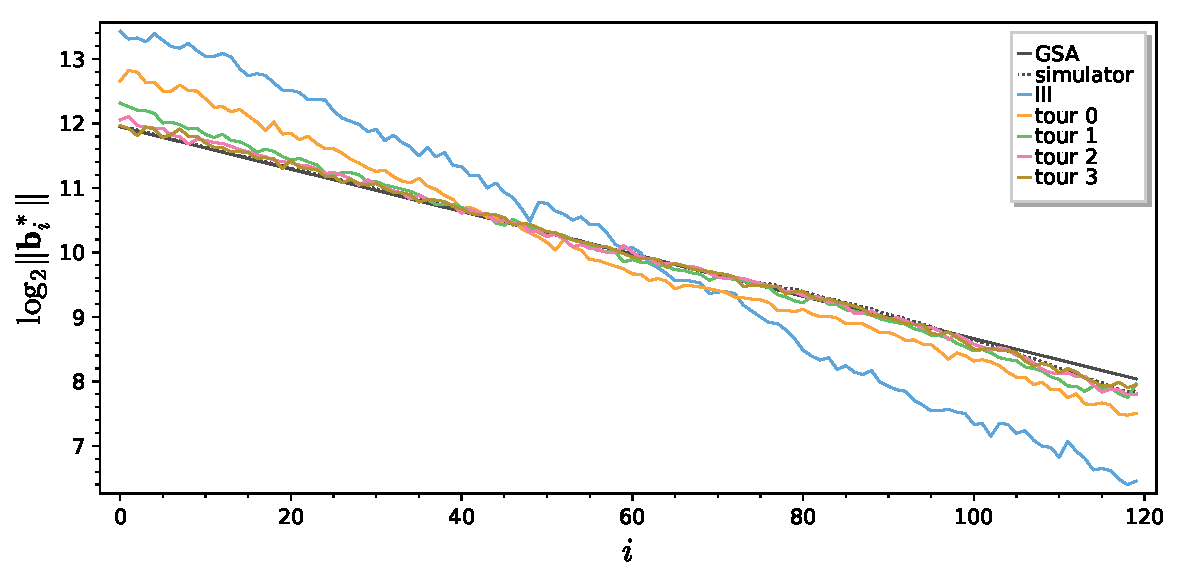
\includegraphics[width=1.0\textwidth]{./bkz-quality.pdf}
\end{center}
\end{center}
\end{frame}

\begin{frame}[label={sec:org829048c}]{Number of Tours}
\begin{scriptsize}
\begin{center}
\begin{tabular}{rrrrrr}
\textbf{Scheme}      / & \textbf{Kyber} & \textbf{Lima} & \textbf{R EMBLEM} & \textbf{NTRU HRSS} & \textbf{SNTRU’}\\
\textbf{Cost Model} &  &  &  &  & \\
\hline
\(0.292\beta\) & 180 & 218 & 112 & 136 & 155\\
\rogr \(0.292\beta + 16.4\) & 196 & 234 & 129 & 152 & 171\\
\rogr \(0.292\beta + \log(8d) + 16.4\) & 210 & 248 & 142 & 165 & 184\\
\enumlinfit{} \(+ 7\) & 456 & 587 & 242 & 313 & 370\\
\enumquadfit{} \(+ \log(8d) + 7\) & 535 & 722 & 270 & 350 & 410\\
\end{tabular}

\end{center}
\end{scriptsize}

After 4 to 8 tours the output does not change much. Thus, some authors write \(8d \cdot t_{SVP}\). Others argue that we need to call the SVP oracle at least once and write \(t_{SVP}\).

\begin{block}{Open Question}
\(8d\) is too large \footfullcite{RSA:LiuNgu13} but it is not clear how far this factor can be reduced in practice.
\end{block}
\end{frame}

\section{Solving SVP}
\label{sec:orgc904ac4}
\begin{frame}[label={sec:orgc6f5b46}]{Solving SVP}
\begin{scriptsize}
\begin{center}
\begin{tabular}{rrrrrr}
\textbf{Scheme}      / & \textbf{Kyber} & \textbf{Lima} & \textbf{R EMBLEM} & \textbf{NTRU HRSS} & \textbf{SNTRU’}\\
\textbf{Cost Model} &  &  &  &  & \\
\hline
\rore  \(0.292\beta\) & 180 & 218 & 112 & 136 & 155\\
\rore \(0.292\beta + 16.4\) & 196 & 234 & 129 & 152 & 171\\
\rore \(0.292\beta + \log(8d) + 16.4\) & 210 & 248 & 142 & 165 & 184\\
\robl \enumlinfit{} \(+ 7\) & 456 & 587 & 242 & 313 & 370\\
\robl  \enumquadfit \(+ \log(8d) + 7\) & 535 & 722 & 270 & 350 & 410\\
\end{tabular}

\end{center}
\end{scriptsize}


\begin{columns}[t]
\begin{column}{0.5\columnwidth}
{\color{LightRed} \textbf{Sieving} }


\begin{itemize}
\item Produce new, shorter vectors by considering sums and differences of existing vectors
\item \textbf{Time:} \(2^{\bigO{\beta}}\)
\item \textbf{Memory:} \(2^{\bigO{\beta}}\)
\end{itemize}
\end{column}

\begin{column}{0.5\columnwidth}
{\color{DarkBlue} \textbf{Enumeration} }

\begin{itemize}
\item Search through vectors smaller than a given bound: project down to 1-dim problem, lift to 2-dim problem …
\item \textbf{Time:} \(2^{\bigO{\beta \log \beta}}\) or \(2^{\bigO{\beta^2}}\)
\item \textbf{Memory:} \(\poly[\beta]\)
\end{itemize}
\end{column}
\end{columns}
\end{frame}

\begin{frame}[label={sec:orgce11613}]{Enumeration Estimates}
Both estimates extrapolate the same data set

\begin{tikzpicture}
    \begin{axis}[xmin=100,height=0.4\textwidth]
      \addplot table [x=d, y=Chen13, col sep=comma]{data/cn11-simulations.csv};
      \addlegendentry{simulation \cite{PhD:Chen13}};
        \addplot+ [domain=100:350, samples=250]{0.000784*x^2 + 0.3667*x - 6.1};
        \addlegendentry{\enumquadfit};
        \addplot+ [domain=100:350, samples=250]{0.187*x*log2(x) -1.019*x + 16.1};
        \addlegendentry{\enumlinfit};
    \end{axis}
  \end{tikzpicture}
\end{frame}

\begin{frame}[label={sec:org7268b40}]{Extended Enumeration Simulation}
Both estimates compared to our simulation

\begin{tikzpicture}
  \begin{axis}[xmin=100,height=0.4\textwidth]
    \addplot table [x=d, col sep=comma, y expr = log2(\thisrowno{2})]{data/fplll-simulations,qary.csv};
    \addlegendentry{FP(y)LLL simulation};
    \addplot+ [domain=100:350, samples=250]{0.000784*x^2 + 0.3667*x - 6.1};
    \addlegendentry{\enumquadfit};
    \addplot+ [domain=100:350, samples=250]{0.187*x*log2(x) + -1.019*x + 16.1};
    \addlegendentry{\enumlinfit};
  \end{axis}
\end{tikzpicture}
\end{frame}

\begin{frame}[label={sec:orgb91cacd}]{Enumeration Simulation vs Experiments}
\begin{tikzpicture}
  \begin{axis}[height=0.4\textwidth]
    \addplot table [x=d, col sep=comma, y expr = log2(\thisrowno{2} * 3.3 * 10.0^9/100.0)]{data/fplll-observations,qary,one-tour.csv};
    \addlegendentry{FP(y)LLL: running time};
    \addplot table [x=d, col sep=comma, y expr = log2(\thisrowno{3}+1 )]{data/fplll-observations,qary,one-tour.csv};
    \addlegendentry{FP(y)LLL: visited nodes};
    \addplot table [x=d, col sep=comma, y expr = log2(\thisrowno{2}), select coords between index={0}{97}]{data/fplll-simulations,qary.csv};
    \addlegendentry{FP(y)LLL simulation};
  \end{axis}
\end{tikzpicture}

\begin{center}
assuming 1 node \(\approx\) 100 cpu cycles
\end{center}
\end{frame}

\begin{frame}[label={sec:org33987a5}]{Enumeration Wors-Case Complexity}
\begin{scriptsize}
\begin{center}
\begin{tabular}{rrrrrr}
\textbf{Scheme}      / & \textbf{Kyber} & \textbf{Lima} & \textbf{R EMBLEM} & \textbf{NTRU HRSS} & \textbf{SNTRU’}\\
\textbf{Cost Model} &  &  &  &  & \\
\hline
\(0.292\beta\) & 180 & 218 & 112 & 136 & 155\\
\(0.292\beta + 16.4\) & 196 & 234 & 129 & 152 & 171\\
\(0.292\beta + \log(8d) + 16.4\) & 210 & 248 & 142 & 165 & 184\\
\rogr \enumlinfit{} \(+ 7\) & 456 & 587 & 242 & 313 & 370\\
\rogr \enumquadfit{} \(+ 7\) & 535 & 722 & 270 & 350 & 410\\
\end{tabular}

\end{center}
\end{scriptsize}

Known worst-case hardness of Kannan’s enumeration is \footfullcite{C:HanSte07} \[\beta^{1/(2e) \beta + o(\beta)} \approx \beta^{0.1839\, \beta + o(\beta)}\] 

\begin{block}{Open Question}
Can we do better than worst-case hardness inside BKZ?
\end{block}
\end{frame}

\begin{frame}[label={sec:orgcda224f}]{Sieving vs Enumeration}
\begin{scriptsize}
\begin{center}
\begin{tabular}{rrrrrr}
\textbf{Scheme}      / & \textbf{Kyber} & \textbf{Lima} & \textbf{R EMBLEM} & \textbf{NTRU HRSS} & \textbf{SNTRU’}\\
\textbf{Cost Model} &  &  &  &  & \\
\hline
\rore  \(0.292\beta\) & 180 & 218 & 112 & 136 & 155\\
\rore \(0.292\beta + 16.4\) & 196 & 234 & 129 & 152 & 171\\
\rore \(0.292\beta + \log(8d) + 16.4\) & 210 & 248 & 142 & 165 & 184\\
\robl \enumlinfit{} \(+ 7\) & 456 & 587 & 242 & 313 & 370\\
\robl  \enumquadfit \(+ 7\) & 535 & 722 & 270 & 350 & 410\\
\end{tabular}

\end{center}
\end{scriptsize}

\begin{block}{}
Sieving is asymptotically faster than enumeration, but does it beat enumeration in practical or cryptographic dimensions?
\end{block}
\end{frame}

\begin{frame}[label={sec:org35814b5}]{Sieving: G6K}
G6K \footfullcite{ADHKPS19} is a Python/C++ framework for experimenting with sieving algorithms (inside and outside BKZ)
\begin{itemize}
\item Does not take the “oracle” view appealed to earlier but considers sieves as stateful machines.
\item Implements several sieve algorithms\footnote{Gauss, NV, BGJ1 (\fullcite{EPRINT:BecGamJou15}; with one level of filtration)} (but not the asymptotically fastest \footfullcite{SODA:BDGL16}  ones)
\item Applies many recent tricks and adds new tricks for improving performance of sieving
\end{itemize}
\end{frame}

\begin{frame}[label={sec:orga91a887}]{Sieving: SVP}
\begin{center}
\begin{tikzpicture}
    \begin{semilogyaxis}[ylabel=seconds, xlabel=\(\beta\), legend style={fill=}, legend pos=north west, height=0.5\textwidth]
        \addplot+ [only marks] table [x=d, y=FPLLL, col sep=comma]{data/exact-svp.csv};
        \addlegendentry{BKZ + pruned enum (FPLLL)};
        \addplot+ [only marks] table [x=d, y=G6K, col sep=comma]{data/exact-svp.csv};
        \addlegendentry{G6K WorkOut};
    \end{semilogyaxis}
\end{tikzpicture}
Average time in seconds for solving exact SVP
\end{center}
\end{frame}

\begin{frame}[label={sec:org48d0cce}]{Darmstadt HSVP\textsubscript{1.05} Challenges}
\begin{center}
\begin{tikzpicture}
  \begin{axis}[xlabel=\(\beta\),ylabel=\(\log_2(\textnormal{cycles})\),height=0.5\textwidth]
    \addplot table [x=d, col sep=comma, y expr = log2(100*\thisrowno{2}),, select coords between index={0}{50} ]{data/fplll-simulations,svp-challenge.csv};
    \addlegendentry{HSVP\(_{1.05}\) non-parallel enum sim};

    \addplot table [x=d, col sep=comma, y expr = log2(100*\thisrowno{2}), select coords between index={70}{166}]{data/fplll-simulations,qary.csv};
    \addlegendentry{SVP non-parallel enum sim};

    \addplot+ [only marks] table [unbounded coords=discard,x=d, col sep=comma, y expr = %
    log2(\thisrowno{3}*3600*2*10.0^9)%
    ]{data/svp-challenge-observations.csv};
    \addlegendentry{HoF:FK15};

    \addplot+ [only marks] table [unbounded coords=discard,x=d, col sep=comma, y expr = %
    log2(\thisrowno{4}*3600*2*10.0^9)%
    ]{data/svp-challenge-observations.csv};
    \addlegendentry{HoF:KT17};

    \addplot+ [only marks] table [unbounded coords=discard,x=d, col sep=comma, y expr = %
    log2(\thisrowno{5}*3600*2*10.0^9)%
    ]{data/svp-challenge-observations.csv};
    \addlegendentry{G6K};

  \end{axis}
\end{tikzpicture}

Estimated and reported costs for solving Darmstadt SVP Challenges.
\end{center}
\end{frame}

\begin{frame}[label={sec:orgf215ade}]{Sieving: Open Questions}
\begin{itemize}
\item G6K does not support coarse grained parallelism across different machines yet: not clear how exponential memory requirement scales in this regime
\item Practical performance of asymptotically faster sieves still unclear
\item Dedicated hardware …
\end{itemize}
\end{frame}

\begin{frame}[label={sec:orgb4a90e8}]{Quantum Estimates}
\begin{scriptsize}
\begin{center}
\begin{tabular}{rrrrrrr}
\textbf{Type} & \textbf{Scheme}      / & \textbf{Kyber} & \textbf{Lima} & \textbf{R EMBLEM} & \textbf{NTRU HRSS} & \textbf{SNTRU’}\\
 & \textbf{Cost Model} &  &  &  &  & \\
\hline
\rore classical & \(\mathbf{0.292}\beta + \log(8d) + 16.4\) & 210 & 248 & 142 & 165 & 184\\
\rore quantum & \(\mathbf{0.265}\beta + \log(8d) + 16.4\) & 193 & 228 & 131 & 153 & 170\\
\robl classical & \enumlinfit{} & 456 & 587 & 242 & 313 & 370\\
\robl  quantum & \(\mathbf{1/2}\,\)(\enumlinfit{}) & 228 & 294 & 121 & 157 & 187\\
\end{tabular}

\end{center}
\end{scriptsize}

\begin{description}
\item[{{\color{LightRed} \textbf{Sieving} }}] Given some vector \(\vec{w}\) and a list of vectors \(L\), apply Grover’s algorithm to find \(\{\vec{v} \in L \textnormal{ s.t. } \|\vec{v} \pm \vec{w}\| \leq \|\vec{w}\|\}\).\footfullcite{PhD:Laarhoven15}

\item[{{\color{DarkBlue} \textbf{Enumeration} }}] Apply Montanaro’s quantum backtracking algorithm for quadratic speed-up.\footfullcite{EPRINT:AonNguShe18}
\end{description}
\end{frame}

\begin{frame}[label={sec:org84ce3a8}]{Quantum Sieving}
\begin{itemize}
\item A quantum sieve needs list of \(2^{0.2075 \beta}\) vectors before pairwise search with Grover

\item Newer sieves use that the search is structured, Grover does unstructured search
\begin{itemize}
\item Quantum Gauss Sieve \[2^{(0.2075 + \frac{1}{2} 0.2075)\, \beta + o(\beta)} = 2^{0.311\, \beta + o(\beta)} \textnormal{ time},\qquad 2^{0.2075\, \beta + o(\beta)} \textnormal{ memory}\]
\item Classical BGJ Sieve \footfullcite{EPRINT:BecGamJou15} \[\phantom{2^{(0.2075 + \frac{1}{2} 0.2075)\, \beta + o(\beta)} = }2^{0.311\, \beta + o(\beta)}\textnormal{ time}, \qquad 2^{0.2075\, \beta + o(\beta)} \textnormal{ memory}\]
\end{itemize}
\item Asymptotically fastest sieves have small lists and thus less Grover speed-up potential
\end{itemize}
\end{frame}

\begin{frame}[label={sec:org191c4dc}]{A Word on Lower Bounds}
\rowcolors[]{3}{gray!20}{gray!10}

\begin{scriptsize}
\begin{center}
\begin{tabular}{rrrrrrr}
\textbf{Type} & \textbf{Scheme}      / & \textbf{Kyber} & \textbf{Lima} & \textbf{R EMBLEM} & \textbf{NTRU HRSS} & \textbf{SNTRU’}\\
 & \textbf{Cost Model} &  &  &  &  & \\
\hline
classical & \(0.292\beta\) \cite{USENIX:ADPS16} & 180 & 218 & 112 & 136 & 155\\
quantum & \(0.265\beta\) \cite{USENIX:ADPS16} & 163 & 198 & 102 & 123 & 140\\
classical & \(0.123\,\beta\log(\beta) -0.70\beta +  6.1\) \cite{C:ANSS18} & 276 & 358 & 142 & 186 & 224\\
quantum & \(0.061\,\beta\log(\beta) -0.35\beta + 2.6\) \cite{C:ANSS18} & 135 & 175 & 69 & 91 & 109\\
\end{tabular}

\end{center}
\end{scriptsize}

\begin{columns}[t]
\begin{column}{0.5\columnwidth}
These estimates ignore:

\begin{itemize}
\item (large) polynomial factors hidden in \(o(\beta)\)
\item MAXDEPTH of quantum computers
\item cost of a Grover iteration
\end{itemize}
\end{column}

\begin{column}{0.5\columnwidth}
Thus:

\begin{itemize}
\item cannot claim parameters need to be adjusted when these estimates are lowered
\item must be careful about conclusions drawn in these models: some attacks don’t work here but work in reality
\end{itemize}
\end{column}
\end{columns}
\end{frame}


\begin{frame}[label={sec:org82031ef}]{More Open Questions}
\begin{itemize}
\item Many submissions use small and sparse secrets where combinatorial techniques apply. Cost of these not fully understood.
\item (Structured) Ideal-SVP is easier than General SVP on a quantum computer.\footfullcite{EC:CraDucWes17} Ring-LWE (but for a choice of parameters typically not used in practice) is at least as hard as Ideal-SVP, but it is not clear if it is harder, e.g. if those attacks extend.
\item The effect of decryption failures in probabilistic encryption based on LWE not fully understood. Some submissions completely eliminate these.
\end{itemize}
\end{frame}

\begin{frame}[label={sec:orgcff666d},standout]{Fin}
\begin{center}
\Huge \alert{Thank You}
\end{center}
\end{frame}

\begin{frame}[allowframebreaks]{References}
\renewcommand*{\bibfont}{\scriptsize}
\printbibliography[heading=none]
\end{frame}
\end{document}